
%%%%%%%%%%%%%%%%%%%%%%%%%%%%%%
\begin{figure}[!hbtp]
\centering
\label{subfig:sm_ichep2012_comb}
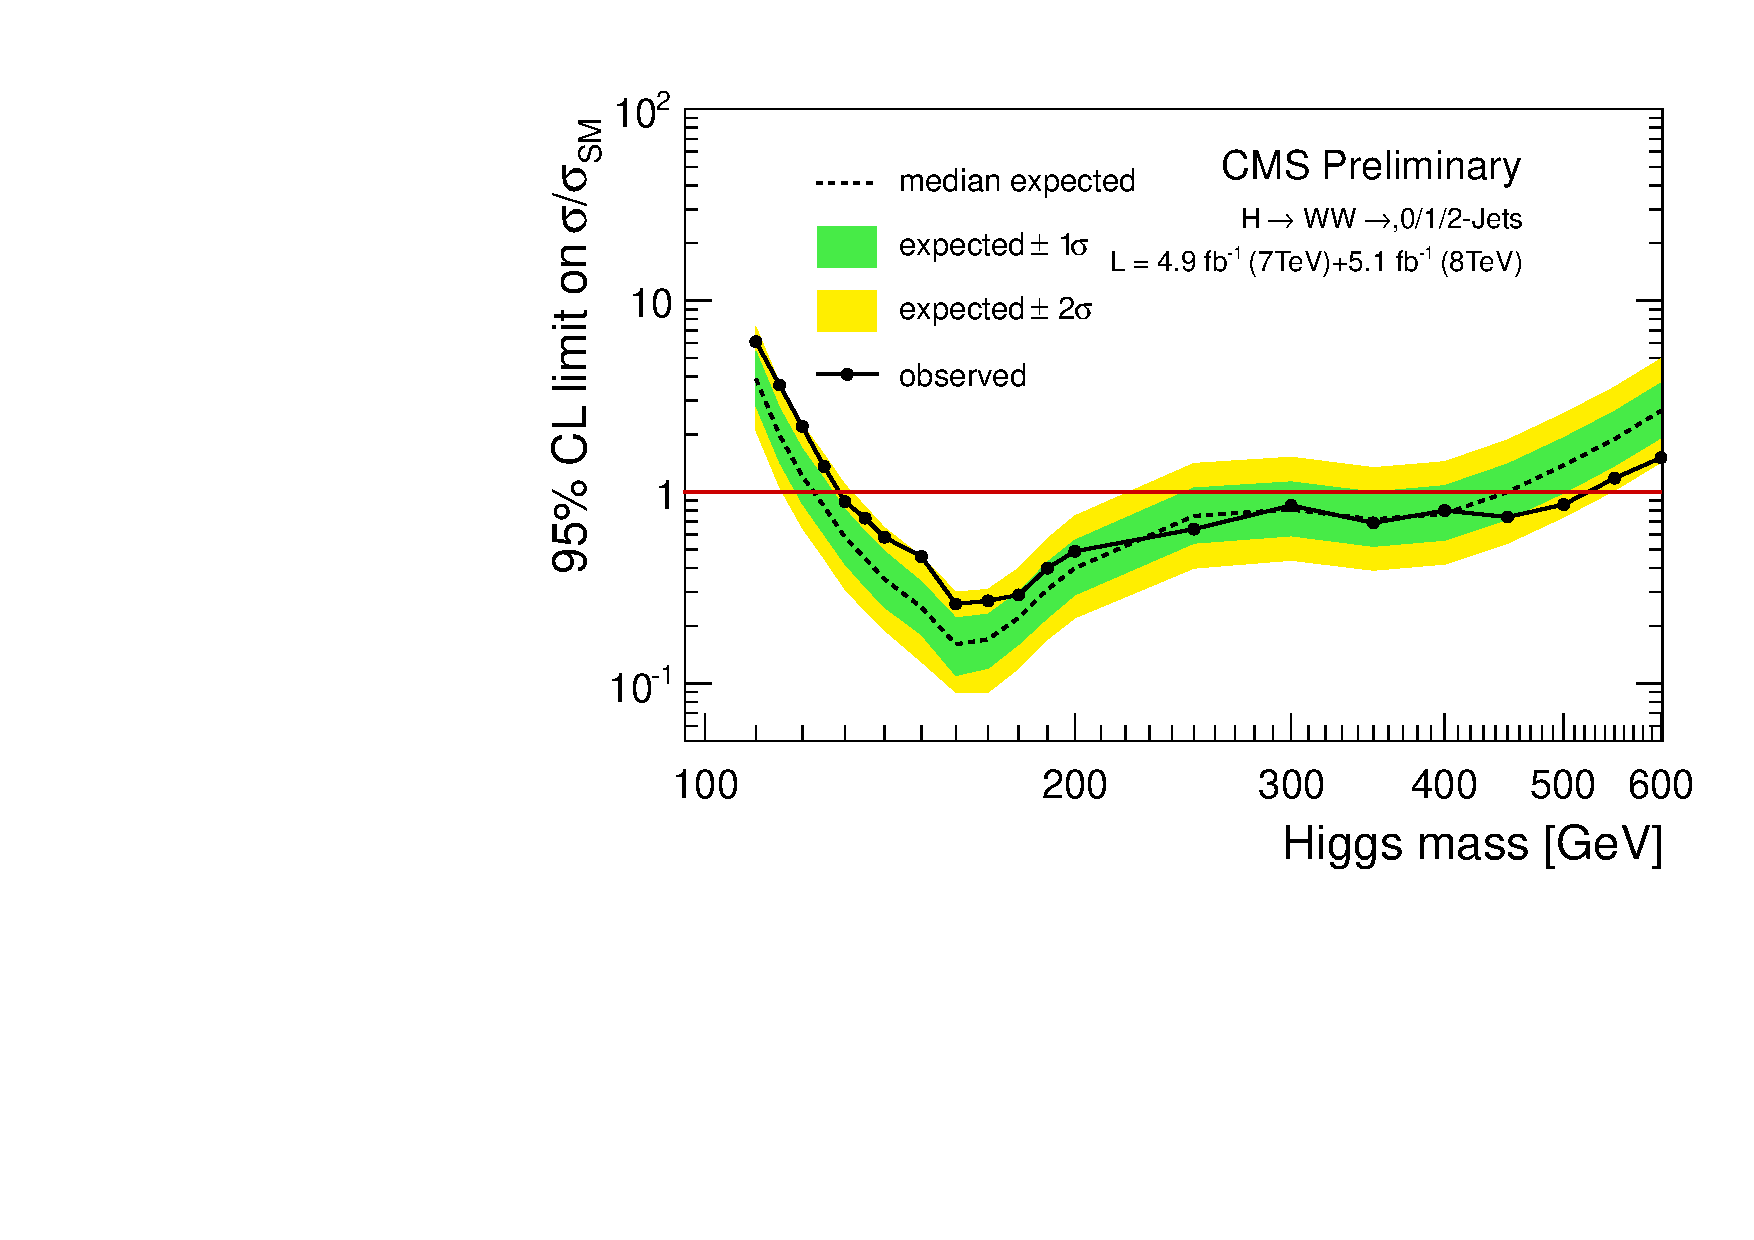
\includegraphics[width=.45\textwidth]{figures/limits_nj_shape7TeV_cut8TeV-CLs-asymptotic_log.pdf}
\label{fig:uls_cut_finalcomb}
\caption{Expected and observed upper limits for SM Higgs using the
  {\bf shape-based} analysis using 7 TeV data, and the cut-based analysis in 8 TeV data. }
\end{figure}

%%%%%%%%%%%%%%%%%%%%%%%%%%%%%%%%%%%%%%%%%%%%%%%%%%%%%%%%%%%%
\begin{table}[hbp!]
\begin{center}
\begin{tabular}{c c c c c}
\hline
\vspace{-3mm} && \\
 Higgs Mass & Observed  & Median expected & Expected range for 68\% & Expected range for 95\%   \\
\hline
\vspace{-3mm} && \\
110 & 6.10 & 3.91 & [2.82, 5.44] & [2.10, 7.29] \\
115 & 3.62 & 1.98 & [1.43, 2.75] & [1.06, 3.69] \\
120 & 2.20 & 1.21 & [0.87, 1.68] & [0.65, 2.25] \\
125 & 1.36 & 0.84 & [0.60, 1.17] & [0.45, 1.57] \\
130 & 0.89 & 0.58 & [0.42, 0.81] & [0.31, 1.09] \\
135 & 0.73 & 0.45 & [0.32, 0.62] & [0.24, 0.84] \\
140 & 0.58 & 0.35 & [0.25, 0.49] & [0.19, 0.65] \\
150 & 0.46 & 0.25 & [0.18, 0.34] & [0.13, 0.46] \\
160 & 0.26 & 0.16 & [0.11, 0.22] & [0.09, 0.30] \\
170 & 0.27 & 0.17 & [0.12, 0.23] & [0.09, 0.31] \\
180 & 0.29 & 0.22 & [0.16, 0.30] & [0.12, 0.40] \\
190 & 0.40 & 0.31 & [0.22, 0.43] & [0.17, 0.57] \\
200 & 0.49 & 0.40 & [0.29, 0.56] & [0.22, 0.75] \\
250 & 0.64 & 0.75 & [0.54, 1.05] & [0.40, 1.41] \\
300 & 0.85 & 0.81 & [0.59, 1.13] & [0.44, 1.52] \\
350 & 0.69 & 0.72 & [0.52, 1.00] & [0.39, 1.34] \\
400 & 0.80 & 0.77 & [0.56, 1.08] & [0.42, 1.44] \\
450 & 0.74 & 1.00 & [0.72, 1.40] & [0.54, 1.87] \\
500 & 0.86 & 1.38 & [0.99, 1.92] & [0.74, 2.57] \\
550 & 1.18 & 1.89 & [1.37, 2.64] & [1.02, 3.53] \\
600 & 1.51 & 2.66 & [1.92, 3.71] & [1.43, 4.97] \\
\hline
\end{tabular}
\caption{Expected and observed upper limits for SM Higgs using the
  {\bf shape-based} analysis corresponding to $\intlumiSevenTeV$ at 7 TeV and the 
{\bf cut-based} analysis in $\intlumiEightTeV$ at 8 TeV data.}
\label{tab:shape7tev_cutbase8tev_uls}
\end{center}
\end{table}
%%%%%%%%%%%%%%%%%%%%%%%%%%%%%%
